% Example template for using the unmeethesis style
% This example is for a Master's candidate in Mathematics
% It contains examples of front matter and most sections that the
% typical graduate student would need to include
% By: N. Doren 02/10/00
%     Minor mods by N. Doren 08/26/11

% Use the following specification for BOTTOM page numbering:
\documentclass[botnum, fleqn]{unmeethesis}
% OR
% Use the following specification for TOP page numbering:
% \documentclass[fleqn]{unmeethesis}




\usepackage{amsmath}
\usepackage{hyperref}
\usepackage{algorithm}
\usepackage{graphicx}
\usepackage[noend]{algpseudocode}
%\usepackage{minted}
\usepackage{minted}
\usepackage{csquotes}
\usepackage{placeins}


\makeatletter
\def\BState{\State\hskip-\ALG@thistlm}
\makeatother

\begin{document}

  \frontmatter

  % Uncomment the next command if you see weird paragraph spacing:
  % That is, if you see paragraphs float with lots of white space
  % in between them:

  %\setlength{\parskip}{0.30cm}

  \title{Distributed Video Analysis for the  Advancing  \\
  Out of School Learning in Mathematics and Engineering Project}

  \author{Cody Wilson Eilar}
  \degreesubject{M.S., Computer Engineering}
  \degree{Master of Science \\ Computer Engineering}
  \documenttype{Thesis}
  \previousdegrees{B.S., University of New Mexico, 2010}
  \date{July, \thisyear}

  \maketitle

  %\makecopyright
  %Copyright page is no longer necessary D. Murrell


  \begin{acknowledgments}
    \vspace{1.1in}
    I would like to thank my advisor, Professor Marios Pattichis, for his
    continuous support in reviewing my source code and for helping me shape my
    ideas for this thesis. I would also like to thank Elmyra Grelle for helping
    me stay on track with all the necessary requirements to graduate. Finally, I
    would like to thank Sandia National Laboratories for supporting me
    financially in my academic endeavors.
  \end{acknowledgments}

  \maketitleabstract %(required even though there's no abstract title anymore)

  \begin{abstract}
    This thesis introduces a distributed processing system for analyzing videos
    acquired through the advancing out of school learning in mathematics and
    engineering \\ (AOLME)
     project. The proposed architecture is demonstrated by
    detecting writing and typing activities based on the Video Analysis (ViDA)
    system. VIDA leverages Amazon Web Services (AWS) to optimally distribute
    segments of video to a heterogenous compute cloud consisting of machines
    that have both CPU and GPU processing hardware onboard. The master node is
    responsible for distributing the videos and the slave nodes perform feature
    reduction on the videos by calculating a handful of cumulative distribution
    functions (CDF) to then be returned to the master for classification using a
    support vector machine (SVM). This thesis will demonstrate the accuracy,
    scalability and flexibility of ViDA for videos collected through AOLME.
    Furthermore, this thesis delves into the architectural details essential to
    distributed video processing on cloud infrastructures.

    \clearpage %(required for 1-page abstract)
  \end{abstract}

  \tableofcontents
  \listoffigures
  \listoftables

  \begin{glossary}{Longest  string}
    \item[$a_{lm}$]
    Taylor series coefficients, where $l,m = \{0..2\}$
  \end{glossary}

  \mainmatter

  % Include the topic chapters
  \chapter{Introduction}
There is strong interest in the development of distributed video analysis
systems that can be used to analyze large video databases. Unfortunately, the
overwhelming majority of software packages for automated video analysis, are not
necessarily designed to scale in order to handle processing on vast video
databases.

An example of a large-scale video database is  provided by the advancing out of
school learning in mathematics and engineering (AOLME) project. AOLME contains
over a thousand hours of high quality video data that need to be analyzed so as
to understand how middle school students acquire basic programming skills.
Currently, most of this analysis is done manually \cite{LopezLeiva2016} to
extract pertinent features for researchers to analyze.

Manual video annotation and transcription is extremely tedious and unsustainable
for large datasets. Because of these inhibitory factors, most of these
encoded videos are left untouched and unanalyzed, potentially leaving thousands
of hours of valuable information about the learning process unexplored and
underutilized.  Clearly there is a need for a tool to aid researchers in
properly analyzing these video datasets efficiently.

\section{\label{section:motivation}Motivation}

Current methods in video analysis systems are extremely application dependent
and are inadequate computationally to sufficiently
investigate video datasets at such a large scale. As such, there is a propensity
for a system that is accurate, scalable and flexible in nature to handle a
variety of challenges in automated video analysis.

Computationally, there is clearly a need for video analysis methods that can be
efficiently implemented in heterogenous compute hardware (such as GPUS and
CPUS), and have said hardware function in a distributed environment. Being able
to leverage heterogenous computer hardware greatly increases the efficiency and
speed of certain, heavily used, video processing algorithms such as 2D
convolutions. Furthermore, having this system exist in a distributed environment
will greatly speed up ephemeral operations and makes it possible to scale up to
address large scale problems. Thus this thesis is motivated by the challenges
associated with analyzing large scale video databases.

\section{\label{section:thesis_statement}Thesis Statement} The thesis of this
research is that it is possible to scale, accurately classify and process videos
using our proposed video analysis architecture for human activity recognition.
The basic idea is to effectively distribute the computation among compute nodes
and collect the results in the master node. The focus is to pre-compute the
computationally intensive feature extractions such as Farneback, Lucas-Kanade
optical flow and SVMs powered by a highly scalable computing architecture, and
exposing those features to researchers so that classification algorithms can  be
developed much quicker and in an interactive way. We show that large amounts of
video data can be accurately classified and that our technique is scalable.
Figure \ref{fig:typing_writing} illustrates the types of pre-cropped videos that
we are attempting to classify.

\begin{figure}[h]
  \label{fig:typing_writing}
  \centering
  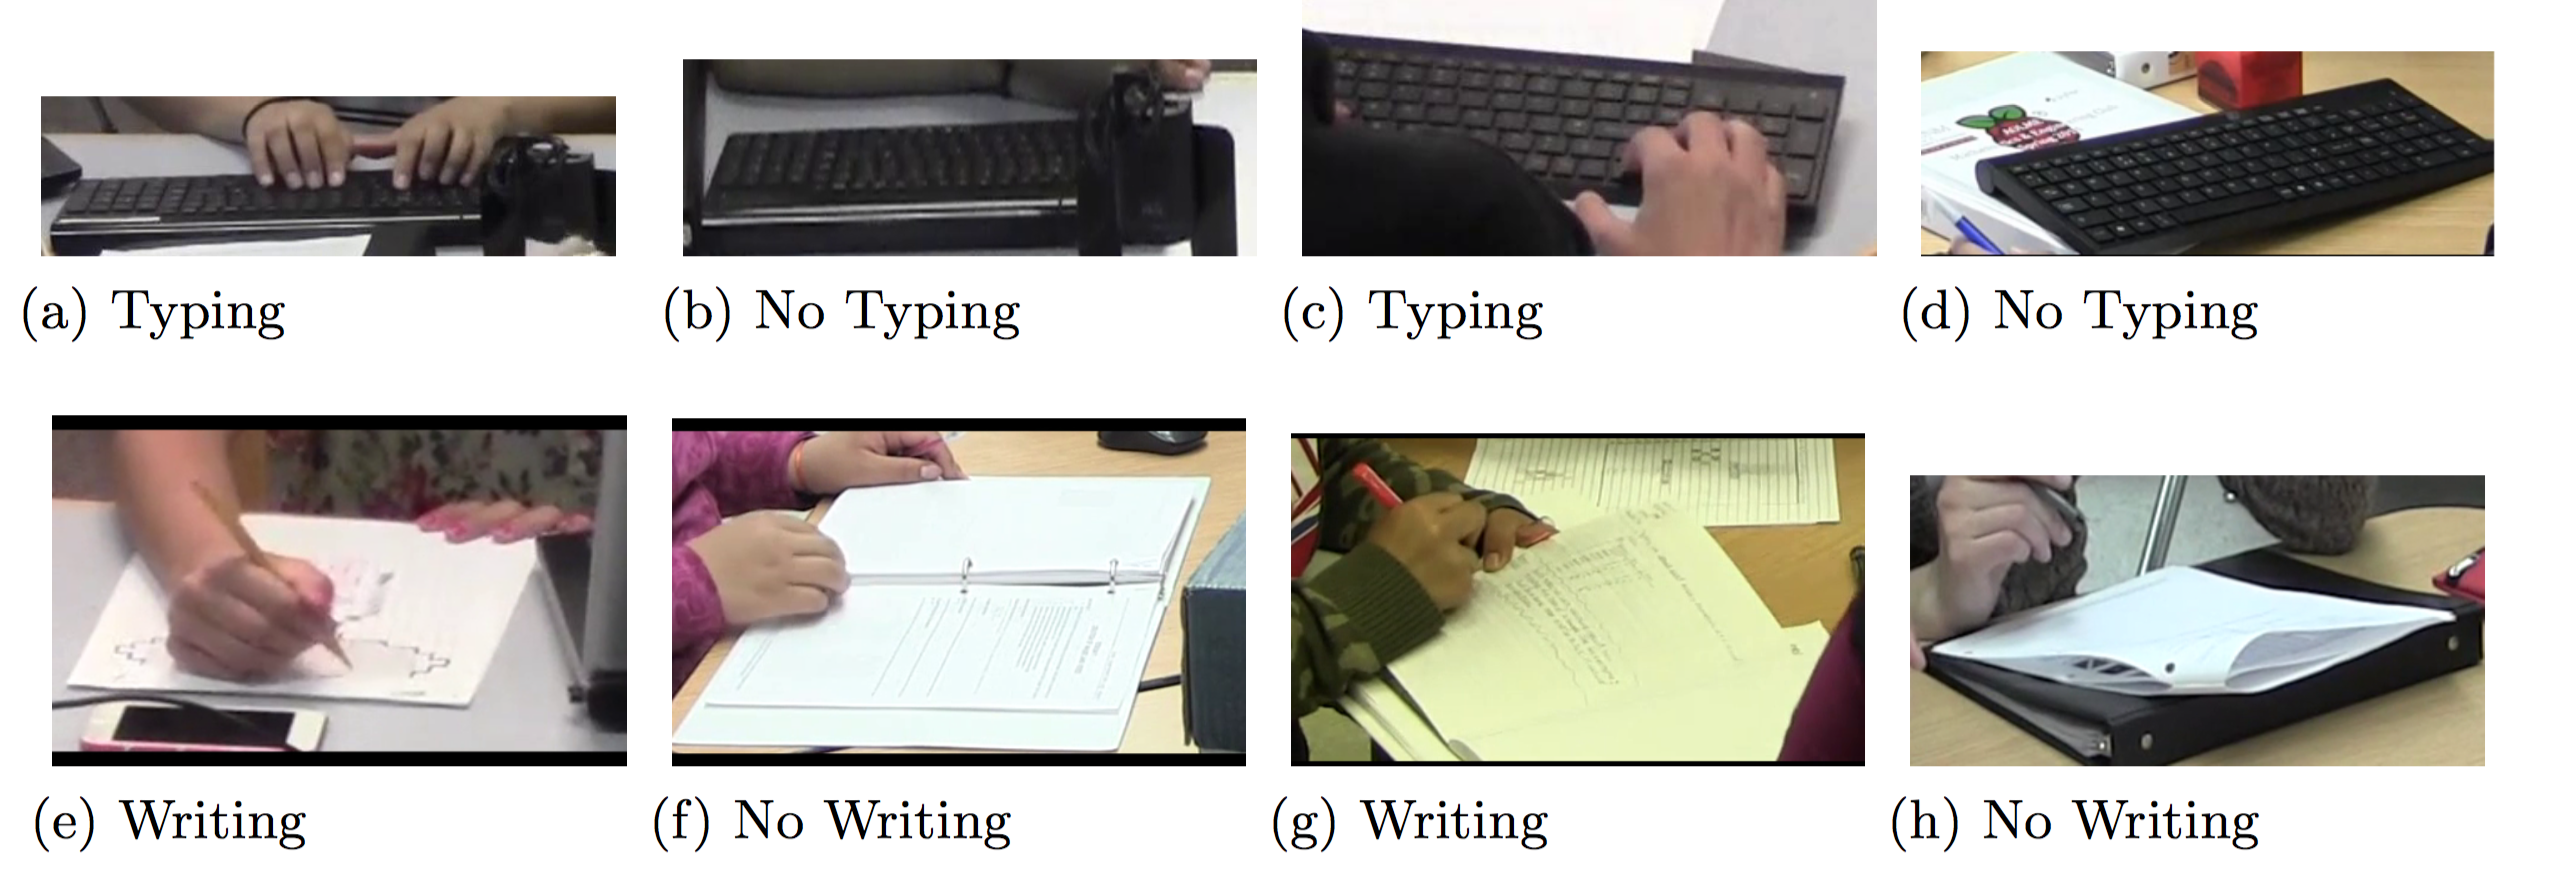
\includegraphics[width=\textwidth]{figures/typing_writing_clip}
  \caption{Example of features that have been manually extracted from the dataset
  for training and testing. For the above example, we need to classifiers for each
  activity to determine if the activity is being performed, or it is not.}
\end{figure}

\section{\label{section:contributions}Contributions}
This thesis contributes to the computer engineering community by providing both
algorithms and an architecture for efficient, scalable and rapid processing of
extremely large video datasets in a cloud environment. Additionally, all
the code written for this thesis is distributed under the MIT open source license
so that the software can be used freely in the community and will thus facilitate
reproducibility and extensibility in this field of research.

\section{\label{section:summary}Summary}
In this thesis, we show that it is possible to reduce the feature set of
videos on the order of Megabytes down to tens of Kilobytes, and then accurately
classify those features at 90\% as a particular human activity. We also create
an architecture that is capable of scaling to dozens of compute notes, and
potentially hundreds thus making the heavy lifting operations, such as computing
optical flow vectors, a trivial task that can be efficiently performed in the
AWS cloud, thus enabling researchers to extract germane features from videos in a
matter of minutes instead of hours.

  \chapter{Background}
Human activity classification in videos is not only a difficult problem to solve
algorithmically but also pushes current computing solutions to the edge of their
capability, especially when attempting to keep up with real-time video rates.
Many possible solutions have been proposed for robust activity classification in
videos \cite{niebles2010modeling} \cite{bashir2007object}
\cite{ribeiro2005human} \cite{karpathy2014large}. Methods such as
\cite{bashir2007object} rely on principal component analysis (PCA) and hidden
Markov models (HMMs) to attempt to classify motions using trajectories; however,
all the datasets study consist of hardware augmentation (a motion tracking glob for
example), used to track motions of hands etc, and do not rely solely on the
video source for classification. Other methods such as
\cite{niebles2010modeling}, use similar techniques that are done in this thesis,
however they do not address the computational burden of producing a histogram of
features to use for classification. Finally, new deep learning methods such as
convolutional neural networks are also gaining popularity in activity
classification in videos because there is no need to select the type of features
\textit{a-priori}, you let the network select what is important for
classification \cite{karpathy2014large}. This technique is computationally
expensive and requires huge amounts of data to properly classify activities
\cite{karpathy2014large}. The study presented by Laptev et al.
\cite{laptev2008learning} showed that it is possible to reduce a video dataset
size significantly using optical flow and using a technique called bag of
features (BoF) which is ultimately used by a machine learning algorithm, such as
non-linear support vector machines to classify the activities. The BoF
technique, however, lacks scalability and proposes no solution to this problem.

Thus we have defined some of the important research in this area and where it is
lacking. In the following sections, we explore important algorithms that are
foundational to the success of our classification and scalable architecture. In
section \ref{section:optical_flow} we review optical flow and how it can be used
for classification and then in section \ref{section:cloud_computing} we explore
the current state-of-the-art cloud computing techniques and how they can be
utilized to create a flexible and scalable architecture.


\section{\label{section:optical_flow}Optical Flow}
There are many varieties of algorithms that aid in the analysis of motions in
videos.  Farneback, Lucas-Kanade and Horn-Schunck \cite{horn1981determining} are
all well studied and successful algorithms for this analysis. In this paper
though, we have chosen to limit the scope to two optical flow methods that are
available to a variety of languages. We explain the implementation of the
Farneback optical flow algorithm \cite{farneback2003two}, also known as dense
optical flow, and the pyramidal, Lucas-Kanade approach to optical flow
\cite{bouguet2001pyramidal}.

\subsection{\label{section:optical_flow_methods}Optical Flow Methods}
In this thesis we attempt to classify two types of activities in video,  typing
and writing. Since both of these activities involve motion, i.e. a change of
apparent structure position from one video frame to the next, optical flow
algorithms  are a suitable tool for attempting to extract germane features from
the video.

We use both Lucas-Kanade \cite{lucas1981iterative} and the Farneback
\cite{farneback2003two}  optical flow algorithms to attempt to extract
important motion features from the AOLME videos. Both algorithms attempt to solve
a common problem known as the \textit{aperture problem}. The problem is defined
by assuming that there have been small changes in both the $x$, $y$ and time components
of a video scene. This is outlined in Equation \ref{eq:delta_image}
Equation \ref{eq:delta_image}

\begin{equation}
I(x,y,t) = I(x+dx, y+dy, t+dt)
\label{eq:delta_image}
\end{equation}

where $I$ is the the image, $x$ \& $y$ are the column row coordinates
respectively, and $t$ is the time between two adjacent image frames. Taking the
Taylor series expansion of Equation \ref{eq:delta_image} results in Equation
\ref{eq:taylor_expansion}


\begin{equation}
f_x u + f_y v + f_t = 0
\label{eq:taylor_expansion}
\end{equation}

where

\begin{equation}
f_x = \frac{\partial f}{\partial x} \; ; \; f_y = \frac{\partial f}{\partial y} \\
u = \frac{dx}{dt} \; ; \; v = \frac{dy}{dt}
\label{eq:taylor_expansion_partial}
\end{equation}

 Equation is \ref{eq:taylor_expansion_partial} is known as the Optical Flow
 equation. The object is to determine what $u$ and $v$ are given that $f_x$ and
 $f_y$ are the image gradients and $f_t$ is the time gradient. Since in Equation
 \ref{eq:taylor_expansion} we have only two unknowns, we cannot solve the system
 without additional constraints. This is known as the \textit{aperture problem}.
 Both the Lucas-Kanade method and the Farneback method attempt to estimate this
 problem. Lucas-Kande attempts to reframe the problem such that we have an
 overdetermined system, solving it and then providing motion vectors for only
 features that move. The Farneback solution, on the other hand, argues that is
 possible to solve the \textit{aperture problem} by first approximating each
 neighborhood of both frames with quadratic polynomials, and then estimating the
 displacement fields between the frames using polynomial expansion. Rather than
 providing only a few motion vectors, the Farneback method provides dense
 optical flow. That is to say that there is a motion vector for every pixel
 between the frames \cite{farneback2003two}.

\subsection{\label{subsection:lucas_kanade} Lucas-Kanade Method}
We leverage a common C++ library that has already implemented a specialized
version of the general Lucas-Kanade algorithm which uses pyramids to solve the
optical flow at different scales of motion \cite{bouguet2001pyramidal}. This
algorithm is provided freely in a C++ computer vision library known as OpenCV
\cite{itseez2015opencv}. Essentially, this algorithm is much like the original
paper published by Lucas and Kanade, but it solves the issue of large motions
between frames and at different scales. By definition, the Lucas-Kande method
assumes that the displacement of features in the image between two frames is
small and roughly constant within a pixel neighborhood. This algorithm, then, by
definition cannot handle large motions between frames, and hence the algorithm
presented in \cite{bouguet2001pyramidal} attempts to more robustly solve optical
flow. The Lucas-Kanade method in OpenCV is often used with Shi-Tomasi
\cite{shi1994good} detection points to estimate what are good features to track
in a frame. This allows the Lucas-Kanade algorithm to perform calculations on a
sparse matrix rather than computing dense optical flow.

\subsection{\label{subsection:farneback_method}Farneback Method} Again, we
leverage the C++ OpenCV library to calculate the motion vectors for Farneback
optical flow. Unlike the previous method, the Farneback algorithm does not
require any track points to estimate motion vectors because it is a dense
optical flow algorithm, i.e. 100\% of the pixels has an associated optical flow
vector. The main idea behind calculating the motion vectors in this method, is
to use polynomial expansion for a neighborhood of pixels \cite{farneback2003two}
and then use that estimation to find a global translation between the two
frames. This essentially aids with global background movement so that unique
movements in the foreground can be accurately measured.

\section{\label{section:cloud_computing}Cloud Computing}
Cloud computing has become a common practice among scientists, engineers and
business owners alike for solving computationally expensive problems at a
relative low cost. Cloud computing offers services on demand rather than
provisioning hardware and software ahead of time. This has opened the door to
researchers who require thousands of computers but don't necessarily have the
funds or access to a cluster of their own \cite{armbrust2009above}. Cloud
computing offers a model that is pay as you go, you only pay for what you use.
This contrasts with the traditional way of solving computationally expensive
problems by acquiring hardware and software ahead of time to run on dedicated
machines. This has the advantage that the owner of the hardware has full control
of its resources, but it has the disadvantage of costing a significant amount of
money and there is a chance that the originally allocated hardware is  either
insufficient for the task or is overdone,  therefore wasting money and
computational resources.  At its core, information technology resources are now
a programmable resource in the cloud, rather than one that has to be manually
setup and configured.

The programming model for cloud computing is fundamentally different than
traditional software models. In the traditional infrastructure of computing,
applications ran on servers and often times relied on the state of a particular
server to perform computations \cite{awsbestpractices}. That model must be
broken in order to efficiently develop applications for the cloud. Clearly, not
all applications can be stateless, but the keys is to eliminate as many stateful
components as possible and replace them with stateless ones. When this paradigm
is followed, along with designing software with well defined interface, list
RESTful, it makes creating a scalable, flexible application easy using cloud
service providers \cite{awsbestpractices} and how to make auto deployment a snap
for rapid testing and distribution using container technologies such as docker.

In the following subsections we explore the current state of cloud computing and
what types of applications can leverage a cloud like infrastructure, a high
level overview AWS and a few of the services that can benefit a video processing
application.

\subsection{\label{subsection:in_the_cloud}What's in the cloud?}
In most of the modern cloud architectures such as Amazon Web Services (AWS),
Microsoft's Azure and Google's Cloud Platform, services offered range from
compute power to database solutions. However, the resources that are often
most important are access to compute resources, highly available networks and
redundant and durable storage. With these three resources available, its possible
to create almost any kind of application in a cloud architecture. The idea is
to eliminate servers, and instead replace it with services. Buzzwords
that emerge from this context are software as a service (SaaS), hardware as a service
(HaaS), and X as a service (XaaS) where X can refer to any number common IT
processes.

The compute resources that are provided are simply virtual machines that can be
created programmatically, usually through some kind of application program
interface (API) provided by the cloud company. These virtual machines can
usually be provisioned with almost any kind of operating system that is
supported by the cloud company of choice. As a result, developers can easily
stand up thousands of virtual instances in the cloud with their operating system
of choice with the click of a button, and tear them down just as quickly.

Storage resources are also crucial to effective cloud software development.
Making storage resources highly available has the advantage of there being
no single point of failure in the data and also facilitates fast access to the
data because no one network interface will be throttled on the network. In a
distributed computing sense, this is extremely important so that data can be operated
upon efficiently over potentially thousands of nodes.

Without a well provisioned network, this could be the ultimate bottleneck for
a software package attempting to leverage the cloud. Fortunately, network as a
service (NaaS) is also available in most commercially available clouds. Most
providers will supply very basic networking for free, but then as with most
resources available in the cloud, it is something that can be upgraded, provisioned
and tailored to the developer's desire.

\subsection{\label{subsection:aws}Amazon Web Services}
Amazon Web Services (AWS) is the most mature cloud solution architecture available
to the public. A popular streaming service in the United States, Netflix,
recently moved all of its streaming services to AWS \cite{netflixawsmove}. This is important to note
because Netflix almost exclusively serves streaming video to hundreds of thousands
of customers everyday. It's obvious from this move alone that there is a lot
of potential in AWS for processing videos. Netflix cites many reason as to why
they moved their monolithic video streaming app to hundreds of micro services
that are run on the AWS cloud, but a few that truly stand out are \enquote{scalable
computing and storage needs}, \enquote{service availability}, and \enquote{cost reduction}
\cite{netflixawsmove}. All of these reasons are enough for any academic institution
to begin leveraging the power of micro services and cloud infrastructure.

AWS provides a number of services that are important to scaling ViDA
both horizontally and vertically. Several services that are important to
our video processing paradigm are:
\begin{itemize}
\item Elastic compute cloud (EC2) - These are virtual machines that can be provisioned
quickly and can be configured a number of ways. They are the work horses for
operating effectively on the AWS cloud. Furthermore, you can provision one, a thousand,
or have them created as you begin to saturate existing instances.
\item Simple storage service (S3) - This services provides storage that is enormous,
durable and distributed over regions in the united states. Petabytes of data can
be easily accessed from anywhere within an Amazon region and have the advantage
of being redundant and fault tolerant. That is to say, the data is not simply
stored on a hard drive at amazon, but is replicated over hundreds of machines
and locations.
\item Simple queue service (SQS) - Is a distributed queue that allows asynchronous
reads and writes to any node in a cluster that has access. This service allows
extremely reliable communication between micro services.
\item Amazon Auto Scaling (AAS) - Auto scaling is a service that allows users
to scale their EC2 instances automatically based on CPU and memory saturation. It
is a key service that allows users to keep costs low yet perform at maximum
capability.
\item Elastic container service (ECS) - This services provides orchestration for
automatic deployment of containers. This is an especially useful service if
your application is deployed into a Docker container.
\end{itemize}

The list provided is by no means meant to be exhaustive, but rather provide
a brief summary of the services that are important to creating an application
that can be horizontally scaled on the cloud. AWS offers dozens of services, each
one can be tailored to the specific needs of the developer and the application
requirements.

EC2 instances are the work horses in the Amazon cloud. Not only are they important
for horizontal scalability, but they are also important for vertical scalability.
There are a number of instance types that can be chosen for customized
applications needs. For example, instances can be provisioned with a single CPU
of moderate frequency and several hundred MBs of random access memory (RAM) or
they can be vertically scaled to contain state-of-the-art GPUs with dozens of
CPU cores and hundreds of GBs of RAM. In fact, AWS is one of the few cloud
services providers that does provide access to instances with GPUs, which is
extremely important for video processing algorithms that leverage efficient
GPU algorithms written in CUDA and/or OpenCL. Thus applications can be scaled
vertically and horizontally using these EC2 instances.

\subsection{\label{subsection:docker}Docker}
Over the last two years, Docker has gained significant traction amongst software
developers for application deployment. Docker is a software package that allows
a variety of *nix type machines to run applications developed on a different
platforms to be run natively. For example, if an application was developed to run
on Ubuntu 14.04, a user who has Docker installed on Cent OS 7 will be able to
run that same byte code. This has a significant impact on the way that software
is deployed. With Docker, gone are the days when software had to be compiled on
multiple architectures or having users install hundreds of third
party libraries just to run the release version of the software.

This paradigm has significant advantages for deploying scalable applications
in a cloud infrastructure. The first advantage being that as long as a *nix
machine is being run on an EC2 instance, you can deploy the package to the instance as
fast as it takes to download the docker image. As a result, maintaining packages
on the instance is not needed. All the software needed for the application
is packaged into the docker image. Secondly, ECS makes it a trivial task to deploy
your Docker container to thousands of instances with only a few commands. With
ECS you can start and stop services, orchestrate varieties of instances and
also perform load balancing to ensure that your application is being run at
top performance and not costing exorbitant amounts of money. 

  \chapter{Methods}
In this chapter we review the basic implementation details of our ViDA
framework. We first demonstrate how we use Lucas-Kanade and Farneback optical
flow algorithms to reduce the feature space to only six 25 bin feature vectors.
With that feature space, we outline how to classify the videos using several
well known machine learning algorithms such as K-nearest neighbors and support
vector machines (SVM). Finally, we cover how we designed this system to be
completely horizontally and vertically scalable on the AWS cloud.


\section{\label{section:vida_oflow} Implementing Optical Flow in ViDA}
In our software, we use two OpenCV library calls, \texttt{goodFeaturesToTrack}
and \\
\texttt{calcOpticalFlowPyrLK} to implement the Lucase-Kanade Pyrmidal optical
flow. The first function is used to find features that can be easily tracked
from one frame to the other using the Shi-Tomasi algorithm \cite{shi1994good}.
The next method then calculates the optical flow between the good points using
the pyramidal implementation of the Lucas-Kanade algorithm
\cite{bouguet2001pyramidal}. Algorithm \ref{alg:lk_flow} outlines the general
program flow for calculating motion vectors in ViDA.

\begin{algorithm}
\caption{Calculating Lucas-Optical Flow from Videos}
\label{alg:lk_flow}
\begin{algorithmic}[1]
\Procedure{CalculateVectors}{$frame1$, $frame2$}
  \If{\text{$track\_points\_initialized$}}
  	\State $opticalflow \gets \texttt{calcOpticalFlowPyrLK}(track\_points, frame1, frame2)$
  \Else
  	\State $track\_points \gets \texttt{goodFeaturesToTrack}(frame1)$
	\State $track\_points\_initialized \gets True$
	\State $optical\_flow \gets  \texttt{CalculateVectors}(frame1, frame2)$
  \EndIf
  \Return $optical\_flow$
\EndProcedure
\end{algorithmic}
\end{algorithm}

The algorithm used in ViDA is similar to Algorithm \ref{alg:lk_flow} but
contains fewer steps since there is no need to get good features to track.
In the C++ software, we also implemented Farneback method. The
Farneback implementation is shown in Algorithm \ref{alg:farneback}.

\begin{algorithm}
\caption{Calculating Farneback Flow from Videos}
\label{alg:farneback}
\begin{algorithmic}[1]
\Procedure{CalculateVectors}{$frame1$, $frame2$}
  \State $optical\_flow \gets \texttt{calcOpticalFlowFarneback}(frame1, frame2)$\\
  \Return $optical\_flow$
\EndProcedure
\end{algorithmic}
\end{algorithm}

As can be seen in \ref{alg:farneback}, we don't need any good features to track
because we are calculating the optical flow globally between frames, rather than
selecting a few features. This has the advantage of tracking optical flow objects
that may fail the Shi-Tomasi method for tracking, but because it is no discriminant
in the features, the resulting motion vectors are dense.


\section{\label{section:comparison}Comparison of Methods}
We implemented the Lucas-Kanade method first in our research because in general,
performance is a concern and, as long as not too many features or
too few features are detected, the Lucas-Kanade algorithm will be faster
\cite{de2015choosing}. Despite this fact, we found that our classifier did
not perform as well on features extracted from the Lucas-Kanade method, as it
did using the Farneback method. Hence most of the results in this thesis
have been calculated with Farneback optical flow unless otherwise specified.

\section{\label{section:feature_extraction}Feature Extraction from Optical Flow}
The \texttt{CalculateVectors} function in both Algorithm \ref{alg:lk_flow} and
\ref{alg:farneback} returns several dense matrices that represent the features
that we can extract from the optical flow output. These features are magnitude,
orientation, x direction and y direction of the optical flow features. These are
ultimately the features that we use to train and classify using an SVM. However,
if we had two $N \times M$ video frames as the input, we now have $4 \times N
\times M$ features. Clearly we have not yet reduced the input feature space.
Thus, based on information that we know \textit{a-priori}, we can reduce our
feature space significantly.

In the case of typing and writing, we know we can expect there to be motion from
one frame to the next. We don't know by how much, but we do know that it is not
zero. Using this knowledge, we can then threshold the optical flow vectors that
we get back from Algorithms \ref{alg:lk_flow} and \ref{alg:farneback}. The
threshold value used was empirically calculated from doing multiple runs on the
AOLME videos. We found we got the best results by only retrieving
optical flow vectors with a magnitude greater than 75\% of the max value. The set
of Equations in \ref{eq:optical_threshold} illustrate this idea.

\begin{align}
  \label{eq:optical_threshold}
  \begin{split}
  \mathbf{V} &= (\mathbf{V_x}, \mathbf{V_y}) \\
  \mathbf{V_m} &=
  \begin{cases}
    1, & \text{if } \|\mathbf{V}\| \geq \max( \|\mathbf{V}\|) \times 0.25 \\
    0, & \text{otherwise}
  \end{cases}
  \end{split}
\end{align}

where $\mathbf{V_x}$ and $\mathbf{V_y}$ are the optical flow vectors in the
x and y directions respectively. $\mathbf{V_m}$ is the bit mask that is
then used to extract the subset of data from each of the dense matrices.

\begin{align}
  \label{eq:subset}
  \begin{split}
  \text{Let: } \\
  \|\mathbf{V\prime}\| &= \|\mathbf{V}\| \circ \mathbf{V_m}\\
  \mathbf{V_x\prime} &= \mathbf{V_x} \circ \mathbf{V_m}\\
  \mathbf{V_y\prime} &= \mathbf{V_y} \circ \mathbf{V_m}\\
  \mathbf{\Phi\prime} &= \mathbf{\Phi} \circ \mathbf{V_m}
\end{split}
\end{align}

Using the optical flow bitmask, $\mathbf{V_m}$, we can then extract features
from each one of our dense matrices using the Hadamard product as shown in
Equation \ref{eq:subset}, where $\|\mathbf{V\prime}\|,
\mathbf{V_x\prime},\mathbf{V_y\prime}, \mathbf{\Phi\prime}$ are subset matrices
for the magnitude, x and y direction and orientation respectively. We have now
reduced the feature space somewhat, but depending on the size of the video and the
amount of entropy per frame pair, we could still have a significant amount of
data to process for classification, this idea is especially true for
Farneback optical flow.

In addition to extracting generic vectors from the video, we also add
geometrical centroids, blob orientation and background motion around the blobs
to the optical flow statistics being used for classification. We implement these
methods to attempt to leverage information that could be useful during
classification. In order to calculate the geometrical centroids and orientations
of each blob, we use some well known algorithms available in OpenCV,
\texttt{connectedComponentsWithStats} and \texttt{findContours}
\cite{itseez2015opencv}. \texttt{connectedComponentsWithStats} is a function
that allows us to compute the centroid for each blob of connected pixels. The
input to this function is our binary mask image, $\mathbf{V_m}$. Once we have
all the connected blobs, we can then calculate the orientation of each one of
those blobs using \texttt{findContours} in combination with with
\texttt{fitEllipse}. The full implementation of this algorithm is outlined in
Appendix \ref{ap:centroids}. The final step is to then dilate each blob, and
then retrieve the magnitude of the optical flow in this region. Appendix
\ref{ap:dilate}. Figure \ref{fig:orient_cent} illustrates the idea of acquiring
the centroid and orientation of the blobs from $\mathbf{V_m}$.

\begin{figure}[h]
  \label{fig:orient_cent}
  \centering
  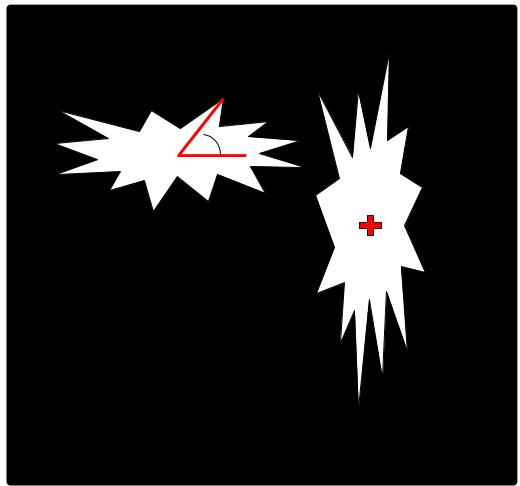
\includegraphics[width=8cm]{figures/cent_and_orient}
  \caption{Example of orientation measurement on the left, and the centroid
  calculation on the right.}
\end{figure}

When the previous optical flow features have been generated, their values are
then organized into a probability density function (PDF) with 25 bins. That is
to say that each frame pair generates a PDF and that PDF is accumulated for
every subsequent frame in the video sequence. When our software reaches the end
of the video file, a normalized, cumulative distribution function (CDF) is
calculated and output for each vector. So for each input video there will be one
CDF with 25 bins for blob orientation, blob centroid x and y, motion vector
magnitude, motion vector orientation and background motion vector magnitude.
Figure \ref{fig:extract_flow} clearly illustrates this concept.

\begin{figure}[h]
  \label{fig:extract_flow}
  \centering
  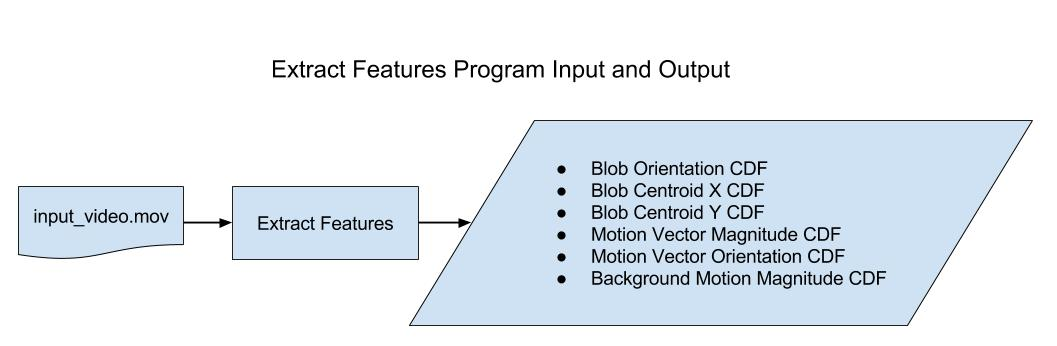
\includegraphics[width=14cm]{figures/extract_features_flow}
  \caption{Flow of the extract features program. For every input video, it will
  return a CDF with 25 bins for each of the extracted features from the motion
  vectors}
\end{figure}

Ultimately, these are the features that are then accumulated for multiple AOLME
videos and used for classification.

\section{\label{section:classification}Classifying the Reduced Feature Space}
At this point we now have accumulated a bag of features for videos. The features
that are collected are stored in a comma separated file (csv) that can be read
in by the any of the popular machine learning packages such as those provided
by the R language or Python's SciKit-Learn. The file contains labels that have
filename, centroid x CDF, centroid Y CDF, background motion CDF, motion magnitude
CDF, motion orientation CDF and classification. We can then use an SVM to classify
the features. To validate our results, we use leave-one-out cross validation
to ensure that we have not overfit the data.

This thesis uses the SVM software that is included in the R language for
accurate classification. The algorithm is based off the original paper written
by Vapnik \cite{cortes1995support} but was then much improved for computational
efficiency by Chang \& Lin in 2011 \cite{chang2011libsvm} with their award
winning software package known as LIBSVM. This library was originally written
in C, but many fans of the algorithm have created software bindings for multiple
languages, including R.

The classification of our feature vectors is very simple since the majority of
the hard work has already been implemented in the machine learning algorithms
we use to do the classification. The process is as follows


\begin{itemize}
  \item Load features from CSV file into an R data frame
  \item Plot statistics about the features
  \item Loop over data frame using leave one out cross correlation
  \item Select most accurate results between K nearest neighbors and tuned, non-linear
  support vector machine.
\end{itemize}

The R code used to do the classification is shown in Appendix
\ref{ap:svm_classification}.

\section{\label{section:distributed_processing}Scalable Architecture}
A core principal for a well designed, horizontally scalable application, is
to design it such that it does not contain state \cite{awsbestpractices}.
When state is required, it the software complexity increases substantially and
makes it difficult to distribute the system over a scalable amount of nodes.
However, if the software was designed such that each service can operate and
stand on its own, it is the perfect embarrassingly parallel computing task to
tackle. For this thesis we focus on ensuring that our feature extractor,
as described in Section \ref{section:feature_extraction}, is completely stateless.
This is a design feature that has allowed us the flexibility to scale our
system over as many nodes as are available on the AWS cloud.

\subsection{\label{subsection:architecture_overview}Architecture Overview}
Our system builds upon AWS to create an easy-to-maintain and easy-to-scale
video processing system. We use S3 storage to put small video clips that
have been extracted from our AOLME dataset. These clips are made available to
to all of the processing nodes. The processing nodes communicate with the master
node using Amazon's simple queue service (SQS). Figure \ref{fig:dataflow} illustrates
the basic distributed system design.

\begin{figure}[h]
  \label{fig:dataflow}
  \centering
  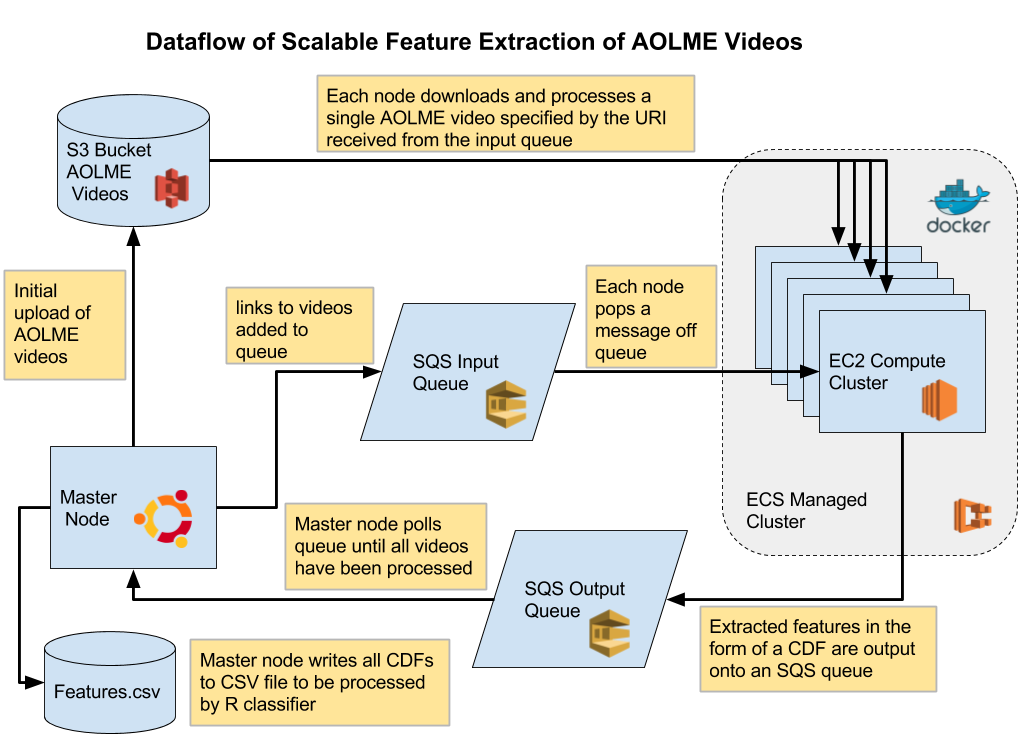
\includegraphics[width=\textwidth]{figures/extract_features_dataflow}
  \caption{Dataflow of the distributed video system using AWS components}
\end{figure}

From Figure \ref{fig:dataflow} we see that the first step is to upload
the videos to S3. We keep the videos very small, because as we show in our experiments
section, it takes quit a long time to process large videos therefore there is a
significant benefit to keeping the video chunks relatively small so that many
machines could potentially work on the feature extraction process. The next step
is to place a message on the SQS queue specifying which video to process and
what its classification is. For the purposes of this thesis, we manually place
messages on the queue so that we can control the flow of messages. In
a production system though, we would have the S3 bucket notify the SQS queue that
a new video was uploaded and ready for processing. The third step is the processing
step. In our setup, we create 20 EC2 instances running our feature extractor application.
Each one of these instances polls the SQS queue waiting for a message to arrive.
As soon as one does, it downloads the appropriate video from the S3 bucket,
processes the video, and then places the results on another SQS queue. At this
point, the master node is polling the results queue and collecting the results
into a csv file. Finally, the csv file can be used to train the SVM in the R
code.

\subsection{\label{subsection:master_node}Master Node Configuration}
The master node in our system is responsible for sending out jobs to process and
then coalescing the results from the calculations performed by the slave nodes.
All of these processes are done using the boto3 \cite{boto3} Python  software
development kit (SDK). The core implementation of AWS uses a  representational
state transfer like (RESTful) interface to communicate to all the services that
Amazon offers in a programatic  way, but they also offer several easy-to-use
object oriented libraries written  in several languages to make programming easier
for the end user. The master node
need not be any specific operating system as long as the Python language
can be interpreted on it. In this thesis, we use Ubuntu 14.04 to run our master
node logic, but it could just as well be OS x or any other flavor of linux.

The master node performs several basic tasks. The first of which is to put
messages on the SQS queue.  This is orchestrated by reading
a csv file that consists of an S3 link to a video segment, the classification of
the segment, the SQS queue to which to output the features and finally the
optical flow method to use. An example of the file is show in Table
 \ref{table:message_queue}.

\begin{table}[h]
  \label{table:message_queue}
  \begin{tabular}{ | l | l | l | p{3cm} |}
  \hline
  \textbf{path} & \textbf{classification} & \textbf{sqs\_queue} & \textbf{of\_algorithm}\\ \hline
  aolme/data/typing/seg\_1.mp4 & 1 & feature\_queue & farneback \\ \hline
  aolme/data/notyping/seg\_1.mp4 & 2 & feature\_queue & farneback \\
  \hline
  \end{tabular}
  \caption{Example of data file that use by the master node to place messages on
  the SQS queue. }
\end{table}

From the example data shown in Table \ref{table:message_queue}, we can see that
the nodes have the ability to switch the algorithm as well as associate a
classification from the video. Having the ability to switch method types allows
us to easily benchmark using Lucas-Kanade optical flow versus Farneback.
We also put the output queue in the message so that the slave nodes know to which
queue to place the results of their calculations. This information is also necessary
for the master to know which queue to wait on to collect all the results. Additionally,
if we need more information to be passed to the slave nodes so that they can
effectively do their job, we can easily put that information in the queue with
the message trivially.

Once the master node has sent all the messages to the queue, it then polls
on the queue it placed the messages on to verify that all the messages have been
remove by the slave nodes. This is an important step to validate that the
slave nodes are indeed popping messages off the SQS queue and processing
the videos that are associated with each message. Once this has been validated,
the master node begins to poll on the designated output queue for the results output
from each of the slave nodes. Once all the results have been collected, the master
node places each of the vectors into a comma separated features file.
The pseudo code for the operations performed by the master are show in Algorithm
\ref{alg:master_node}.

\begin{algorithm}
\caption{Master Node Implementation Pseudo-Code}
\label{alg:master_node}
\begin{algorithmic}[1]
  \State $videos\_to\_process \gets \texttt{ReadInputData(input.csv)}$
  \For{\texttt{i = 0; i < len(videos\_to\_process); ++i}}
    \State $sqs\_message \gets \texttt{CreateMessage(videos\_to\_process[i])}$
    \State $output\_queue\_uri \gets videos\_to\_process[i].output\_queue\_uri$
    \State$\texttt{SendSqsMessage(}sqs\_message, sqs\_uri \texttt{)}$
  \EndFor

  \While{$\texttt{MessagesRemainingInQueue(}sqs\_uri \texttt{)} \neq 0$} \Comment{Poll queue every second}
    \State $\texttt{Sleep(1)}$
  \EndWhile

  \While{$\texttt{MessagesRemainingInQueue(}output\_queue\_uri\texttt{)} \neq 0$}
    \State $feature\_vectors \gets \texttt{ReceiveSqsMessage(output\_queue\_uri\texttt{)}}$
    \State $\texttt{Sleep(1)}$
  \EndWhile

  \State \texttt{WriteFeaturesToDisk(} $feature\_vectors$ \texttt{)}

\end{algorithmic}
\end{algorithm}

As we have shown in this section, very little needs to be configured on the master
node other than the ability to run Python and the AWS python utilities. This
makes running our software from almost any type of machine very easy with just a
few setup steps. The master node plays an important role in sending and receiving
the data that the user wishes to process and is an enabling part of our system.
That is to say, it really doesn't matter what software we are running on our
slave nodes, as long as the slave nodes fulfill the contract that we have
defined in our messaging format. This means that we don't necessarily have to
run our C++ extract features program on the slave nodes, but we could be running
any flavor of algorithm we wish with no configuration changes on the master node.
Not only is this setup scalable, but it's highly flexible because of this idea.

\subsection{\label{subsection:slave_node}Slave Node Configuration }
The next very important piece to our innovative architecture is the algorithm
that is run on all the slave nodes. This algorithm simply polls on a single
queue, then once a messages is received, it downloads the the small S3 video
segment, processes it using our feature extraction technique, puts the results
on a queue that it has discovered on the incoming message, deletes the video
locally and then begins polling on the queue again. Algorithm \ref{alg:slave_node}
illustrates this idea clearly.

\begin{algorithm}
\caption{Slave Node Implementation Pseudo-Code}
\label{alg:slave_node}
\begin{algorithmic}[1]

  \While{$True$}
    \State $sqs\_message \gets \texttt{ReceiveMessages(} queue\_name \texttt{)}$ \Comment{Blocking call}
    \State $video\_path \gets \texttt{DownloadS3Video(} sqs\_message.video\_path \texttt{)}$
    \State $features\_cdf \gets \texttt{ExtractFeatures(} video\_path \texttt{)}$ \Comment{Call C++ Code}
    \State $\texttt{SendS3Message(} sqs\_message.output\_queue, features\_cdf \texttt{)}$
    \State $\texttt{DeleteSqsMessage(} sqs\_message \texttt{)}$ \Comment{Remove message from queue}
    \State $\texttt{Sleep(1)}$
  \EndWhile
\end{algorithmic}
\end{algorithm}

We can see that the slave node logic is, like the master node, very simple. We
simply wait for messages to come in from one queue, process the video, and then
output the features onto another queue. However, there is a piece missing from
Algorithm \ref{alg:slave_node} that makes the slave nodes a truly innovative
part of our overall architecture and that is the orchestration and deployment
of our highly refined C++ code.

One of the big hurdles in launching applications that run on a cluster is that
all the nodes on the cluster must be running the same libraries, operating
system,  and versions of the software so that all the answers are returned from
the slaves are repeatable and reliable. In traditional systems, this action was
typically performed by system admin and as a result, you had to rely on third
party packages and libraries that were deployed with the cluster. So if the
software under development needed some updates to a package or some bug fixes,
you were out of luck. You had  to work around those bug fixes and/or write the
updates by hand to get similar  functionality. This is not so with our system.
Using ECS, EC2 and Docker \cite{Merkel:2014:DLL:2600239.2600241}, we  have
developed a system that allows any flavor of linux to be deployed with any
version of software that is required to run on the slave nodes seamlessly. For
example, we developed our C++ code using OpenCV 3.0 and g++4.8 all on Ubuntu
14.04 and built a Docker container that packaged all that software together.
We were then able to deploy our software to an Amazon machine image (AMI) running
an Amazon flavor of Linux that was built for running docker and for communicating
to an ECS cluster. We did all that without configuring a single Linux instance
by hand. And should we choose to roll back to an earlier version of OpenCV or
upgrade our compiler to the latest standard, we could do so by changing the
configuration of our Docker container and our development environment. This
method in no way hinders either vertical or horizontal scalability. With Docker,
we can still pass flags that allow the container to take over the host's GPUs
so that any code written specifically for the GPUs can still be run in a container.


\section{\label{section:auto_deployment}Automatic Deployment of Software and
the Development Process}
An aspect of this thesis that separates us from many of the techniques proposed
in the background section, is the way we have developed our system to be readily
repeatable, easy to use and flexible to allow to future improvements. This is
especially important to UNM's image and video processing and communication lab
iVPCL lab so that future graduate students can leverage the work done in this
thesis to get a head start on future developments of the proposed feature
extraction algorithm and on ViDA's architecture. In this section we cover
several topics that demonstrate that we have done more than just provide an
innovative solution to classifying activities in video, but have also created a
system after which other projects can model themselves. Specifically, we cover
how ViDA's underlying C++ code is developed and how it is automatically and
seamlessly deployed to AWS all the while maintaining a vertically and
horizontally scalable architecture.

\subsection{\label{subsection:opencv_tapi}Vertical Scalability}
Since the iVPCL is strongly geared towards vertically scalable solutions using
FPGAs and GPUs, it is fitting that we should also make the goal of this thesis
to leverage those technologies. To do so, we have developed our software to take
advantage of OpenCV's transparent API known as TAPI. The transparent API is an
enabling technology to be able to seamlessly switch between GPU, CPU and or any
hardware technologies without the software programmer having to select one at
compile time or at run time explicitly. TAPI uses Open Computing Language
(OpenCL) has its underlying technology to achieve significant improvements over
its base algorithm suite. This fundamental technology allows the programmer to
write software for a variety of hardware implementations without being burdened
with implementing the algorithms by hand. For example, the Farneback optical
flow algorithm that is already provided in the OpenCV library can be run easily
on either the GPU or the CPU with almost no extra programming on the programmers
part. This is also a powerful idea for users who want to distribute software to
wide community, but have hardware accelerations that can be added to speed the
software up when the hardware is available on the system. So if the programmer
has attached an accelerated algorithm for computing the discrete radon transform
as demonstrated in \cite{Cesar2014a}, it is completely possible to plug that
implementation into OpenCL and in turn, program the abstraction layer into the
OpenCV library. This also means that the horizontally scalable aspect of this
thesis still holds so that we can distribute the same algorithm to nodes with
less capable hardware. Although it is optimal to have a cluster of machines with
FPGAs hanging from the PCI express bus, implementing the software in OpenCL
gives users the option to run the code on almost any compute device. This means
that the code can run on machines in AWS or in a local cluster. Furthermore,
machines that have the necessary hardware and are accessible in the lab can
perform some of the heavy lifting before farming out the rest of the data to the
slave nodes on the AWS cloud. So even though the system is designed with
horizontal scalability in mind, the option of going vertically scalable for
certain computations has been in no way hindered.

\subsection{\label{subsection:cont_integration}Continuous Integration}
Its all too often that software is written and completely forgotten about
because the build process is too complicated and burdensome on the users of the
interface.  A goal of this thesis maximize reusability and maintainability. We
accomplish this using a  popular software technique called continuous
integration \cite{duvall2007continuous}. Continuous integration is the idea that
software should be constantly giving developers feedback about the state of
their software to ensure robustness and to have an obvious tool for developers
to use document the build process of the software. This is an especially
important tool for teams of developers so that failures of new commits
can easily be observed quickly and effectively. This has the advantage of addressing
errors early on in the software development phase so that errors are addressed
immediately.

For this thesis, we chose to use an online tool called Travis-CI for our
continuous integration. Travis easily hooks into our Github repository and
automates the build process of our extract features program. The build of our
C++ program consists of compiling and linking against all third party libraries,
running all of our google test unit tests, and then deploying the Docker image
to AWS to be used for deployment on the ECS cluster. This tool significantly
unburdens the developer from having to do these steps manually. Continuous
integration also ensures that the unit tests that have been developed for the
software work on the deployed environment specifically in the docker image. In
other words, we develop the software locally on any flavor of linux,  but there
is a chance that any new changes that we have made to the software do not work
in the deployed system. Travis-CI acts as an automated alert that something might
not be right in the software.

The fact that the continuous integration also pushes our Docker image up to  our
ECS cluster is also huge advantage. This process  ensures that  our Cluster is
always running the latest compiled and unit tested version.  So not only have we
made deployment of our software easy using a Docker  container to package it up,
we've also automated the entire deployment process of our software simply by
pushing our code to our Github repo.

Making the deployment and build of our software automated has guaranteed us
that we will have repeatability in our code and that we have the latest
functioning version running on our compute cluster. Furthermore, if mistakes are
made at the local development level and they are not caught until the developer
has pushed their changes to a Git repo, the automated build system will trigger
a failure and not deploy the system. A key contribution with using the automated
build system is that anyone from anywhere will be able to repeat the experiments
that we have performed in this paper with very little software configuration. We
have essentially frozen the code in a working state. Even if AWS goes away, the
core Docker image is available to be run on any *nix type machine with Docker installed.
So if future users decide that they want to use our extract features algorithm,
it is ready to run. Figure \ref{fig:continuous_integration} illustrates the
general flow of the continuous integration in ViDA.

\begin{figure}[h]
  \label{fig:continuous_integration}
  \centering
  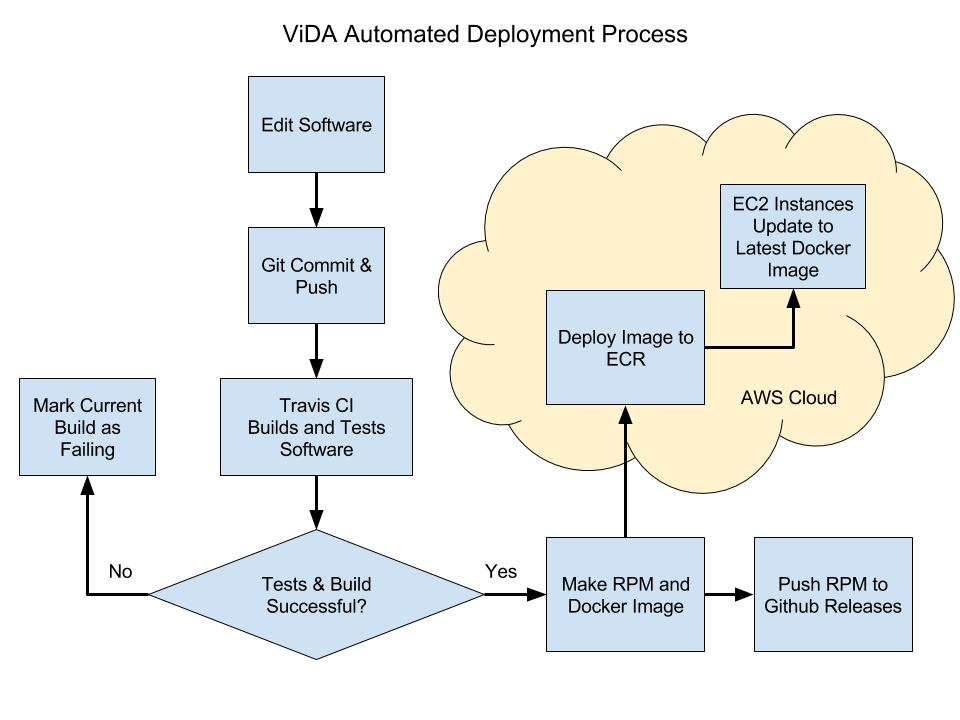
\includegraphics[width=\textwidth]{figures/continuous_integration}
  \caption{Automated deployment of ViDA to the AWS cloud using continuous integration}
\end{figure}

\subsection{\label{subsection:tdd}Test Driven Development}
For the majority of our C++ development, we used a software engineering technique
called test driven development (TDD) \cite{beck2003test}. This technique is germane to
our method's section because repeatability of our experiments and future
extension of our work depends on well developed, robust software. The main idea is that
before we ever wrote code to implement a new algorithm, we first design a failing
test and then write code to make that test pass. This has several advantages over
not writing tests for code:

\begin{itemize}
\item It gives developers a predictable way to code. Rather than thinking
abstractly about what goals a developer is attempting to accomplish, the developer
writes concrete tests that should validate the behavior that is desired.
\item It allows for lessons to be learned early on about the implementation details
of the software. If a developer delves directly into solving a software problem
with a single mindset about how it should be implemented, then the opportunity
for a different design pattern to be used is extinguished. The main idea being
that if test driven development is used for designing an algorithm then the best
design pattern for the problem will be chosen, not just the one the developer
is familiar with.
\item Test driven development forces developers to be accountable. All too often
code is written with the mindset that its okay to commit hundreds or even
thousands of lines of code most of which is barely tested. And thus the code
becomes riddled with bugs and other developers end up having to fix those issues.
With TDD, this is a less frequent occurrence because developers must write a test
for every logical unit of code.
\end{itemize}

For this thesis we use TDD to develop our extract features program and to design
several programs that we use for experimental purposes. In order to facilitate
the development, we use google test as our C++ testing framework
\cite{googletest}. An example of a test we have written to test receiving a
single video frame from a file is shown in Appendix \ref{ap:google_test}. This
test uses a concept fro the TDD community known as a mocked object. The
philosophy behind using a mocked video reader as illustrated in the test, is
that we don't want to design our tests to be reliant on the state of the current
system. If we do so, the second we push our code to the repository, our
continuous integration tool will fail. Mocked objects give us the ability to
test our algorithms without having to rely on the state of our development
machine, the network or other variable elements. This is a powerful concept
because it ensures that our tests run fast and also forces us to program to
interfaces rather than concrete objects. In order to fully leverage the power of
mocked objects, we use a design pattern, as shown Appendix \ref{ap:google_test},
known has dependency injection \cite{gamma1995design}. The idea behind
dependency injection is that we can inject our dependencies into an algorithm at
runtime or compile time to have our object get the resources it needs to perform
a calculation in a variety of ways. For example, in our test in Appendix
\ref{ap:google_test}, we inject the interface called ``Reader''. ``Reader'' is a
specific example of high-performance dependency injection because no virtual
interfaces are used. This concept can only be used at compile time and the
interfaces cannot be swapped out at runtime. High performance dependency
injection is achieved by using only templates, which by their nature, can only
be determined at compile time and not run time. In order to achieve type
inference at runtime, we would need to use a virtual interface instead which has
the additional overhead of doing a virtual table lookup. As a result of using
this reader interface instead of using OpenCV's video reading capabilities, we
give ourselves the flexibility to read from hierarchical data format (HDF5)
files, a web interface, or anything as long as we adhere to the contract we have
defined in the interface code. And thus we can also write a mocked object, which
is to say, an object that we can easily define the inputs and outputs of on the
fly so that we can test a variety of scenarios in our motion estimation
algorithm without having to rely on any external resources. Figure
\ref{fig:hiperf_dependency} illustrates how dependency injection looks for our
MotionEstimation class.

\begin{figure}[h]
  \label{fig:hiperf_dependency}
  \centering
  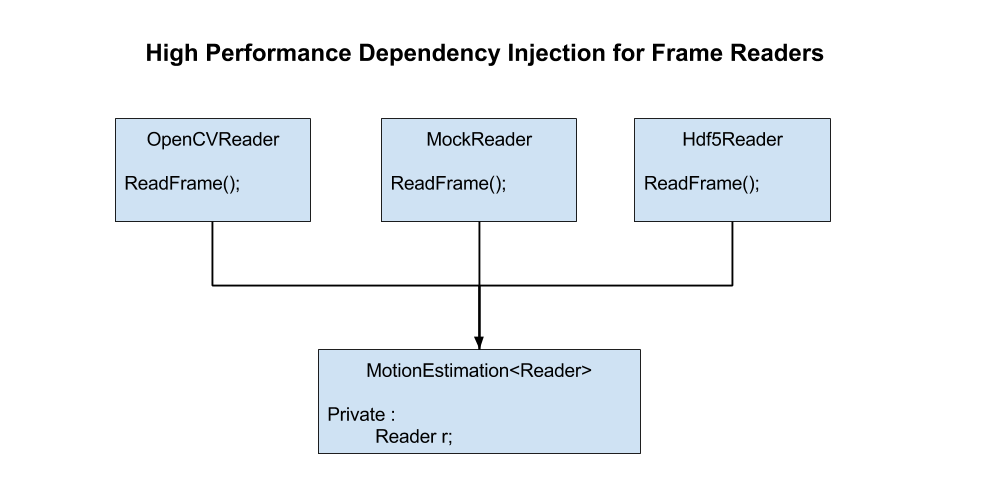
\includegraphics[width=\textwidth]{figures/dependency_injection}
  \caption{High performance dependency injection using templates to implement the
  motion estimation class with different types of video readers.}
\end{figure}

The appendix example demonstrates how we now have a failing test, and we can then
begin implementing the code that causes test to pass. As a result, if we
push our failing test to Github, our current build will not be deployed to the cluster
until we have our tests passing. Figure \ref{fig:passing} illustrates what a commit
looks like when it is passing on our Github project and Figure \ref{fig:passing}
shows what it looks like when the build is failing because of a test, compilation
issues, or problems pushing to the AWS cloud.

\begin{figure}[h]
  \label{fig:passing}
  \centering
  
\includegraphics[width=\textwidth]{figures/passing}
  
\includegraphics[width=\textwidth]{figures/failing}
  \caption{An example of two commits that were pushed to our repository. The
  top figure shows how the build is marked as passing with a green check mark,
  and the bottom shows the build failing with a red x.}
\end{figure}

  \chapter{Results \& Discussion}
\section{\label{section:the_data}The AOLME Dataset}
The AOLME dataset is an enormous repository of over 900 hours of video
recordings of students. The videos contain students
interacting with facilitators, their peers and computers to write code in
Python on the Raspberry Pi.  The dataset is wealth of information but difficult
to exploit in its current state.  The data used for this thesis is a subset of
the entire AOLME dataset. By hand, we have selected several videos and extracted
typing and writing clips from the original dataset and are using these as ground
truth for measuring the accuracy of our methods.

As Figure \ref{fig:typing_writing} suggests, we are only using a cropped version
of the video. The reason for this is that we are not attempting to solve the tracking
problem in this thesis, only the classification problem. Hence, we assume that
the videos entering into our software have already been clipped and cropped with
the target activities inside of them and the corresponding lack of the activity.
Our subset of the AOLME database consists of the following:

\begin{itemize}
\item Twenty videos of typing
\item Twenty videos of no typing
\item Twenty videos of writing
\item Twenty Videos of no writing
\end{itemize}

\section{\label{section:accuracy} Accuracy of Classification}
In this section we explore how well our results are for both the classification
of typing and writing videos using the techniques described in methods chapter.

For our first set of results, we ran to classifying typing motions in videos.
The input messages into the cluster are shown in Table \ref{tab:message_list}.
The original dataset, however, contains 10-20 for each of the training classifications,
we have left them out in this table for brevity.
\begin{table}[h]

  \begin{tabular}{ | l | l | l | p{2cm} |}
  \hline
  \textbf{path} & \textbf{classification} & \textbf{sqs\_queue} & \textbf{algorithm}\\ \hline
  aolme/data/typing/seg\_1.mp4 & 1 & feature\_queue & farneback \\\hline
  aolme/data/typing/seg\_2.mp4 & 1 & feature\_queue & farneback \\\hline
  aolme/data/typing/seg\_3.mp4 & 1 & feature\_queue & farneback\\\hline
  aolme/data/typing/seg\_4.mp4 & 1 & feature\_queue & farneback\\\hline
  aolme/data/typing/seg\_5.mp4 & 1 & feature\_queue & farneback\\\hline
  aolme/data/typing/seg\_6.mp4 & 1 & feature\_queue & farneback\\\hline
  aolme/data/typing/seg\_7.mp4 & 1 & feature\_queue & farneback\\\hline
  aolme/data/typing/seg\_8.mp4 & 1 & feature\_queue & farneback\\\hline
  aolme/data/typing/seg\_9.mp4 & 1 & feature\_queue & farneback\\\hline
  aolme/data/typing/seg\_10.mp4 & 1 & feature\_queue & farneback\\\hline
  \ldots & \ldots & \ldots & \ldots\\\hline
  aolme/data/notyping/seg\_1.mp4 & 2 & feature\_queue & farneback\\\hline
  aolme/data/notyping/seg\_2.mp4 & 2 & feature\_queue & farneback\\\hline
  aolme/data/notyping/seg\_3.mp4 & 2 & feature\_queue & farneback\\\hline
  aolme/data/notyping/seg\_4.mp4 & 2 & feature\_queue & farneback\\\hline
  aolme/data/notyping/seg\_5.mp4 & 2 & feature\_queue & farneback\\\hline
  aolme/data/notyping/seg\_6.mp4 & 2 & feature\_queue & farneback\\\hline
  aolme/data/notyping/seg\_7.mp4 & 2 & feature\_queue & farneback\\\hline
  aolme/data/notyping/seg\_8.mp4 & 2 & feature\_queue & farneback\\\hline
  aolme/data/notyping/seg\_9.mp4 & 2 & feature\_queue & farneback\\\hline
  aolme/data/notyping/seg\_10.mp4 & 2 & feature\_queue & farneback\\\hline
  \end{tabular}
  \caption{Data that is sent to the SQS for calculation on the cluster. The
  original dataset includes 10-20 for both classifications}
  \label{tab:message_list}
\end{table}

Using our R code, we then plot some statistics about the vectors that have come
back from the cluster.
% The first column represents the statistics from videos that have the activity
% in them, and the second column represents the lack of that activity. Just from
% visual inspection, we can already see that there differences in the overall
% statistics, which means that we should have very good luck with our support
% vector machine properly classifying the results.

\FloatBarrier

% \begin{figure}[h]
%   \label{fig:typing_box_whiskers}
%   \centering
%   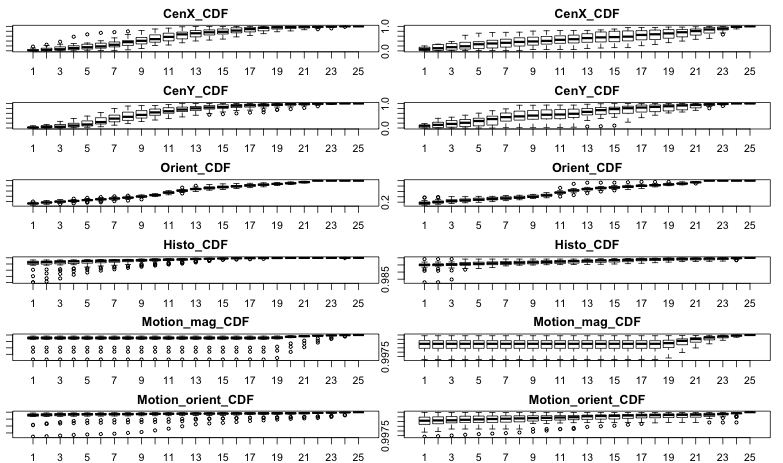
\includegraphics[width=\textwidth]{figures/typing_box_whiskers}
%   \caption{Box and whiskers plot of CDFs for typing. The first column represents the
%   statistics for typing and the second column represents the statistics for no
%   writing.}
% \end{figure}

With those feature vectors, we found that we were able to get the confusion matrix
shown in Table \ref{tab:typing_confusion}
\begin{table}[h]
  \begin{centering}
  \begin{tabular}{| l | l | l |}
  \hline
   & \textbf{typing} & \textbf{no typing}\\ \hline
  \textbf{typing} & 19 & 1 \\ \hline
  \textbf{no typing} & 3 & 17 \\ \hline
  \end{tabular}
  \caption{Confusion matrix for classification accuracy for typing}
  \label{tab:typing_confusion}
\end{centering}
\end{table}

\FloatBarrier

From Table \ref{tab:typing_confusion} we can see that we get 90\% accuracy for
classifying typing motions on the keyboard. We had difficulty classifying
videos that had significant motion in them, but the motion was not typing and
we also found that we had trouble classifying the videos where there is was
not much typing in the videos that were classified as typing. But overall, when the
scene clearly had typing and when it clearly did not, we found that we had
90\% accuracy.

Our results for determining writing, however, were not as good as our results
for classifying typing. Our CDFs for typing are shown in figure

% \begin{figure}[h]
%   \label{fig:typing_box_whiskers_1}
%   \centering
%   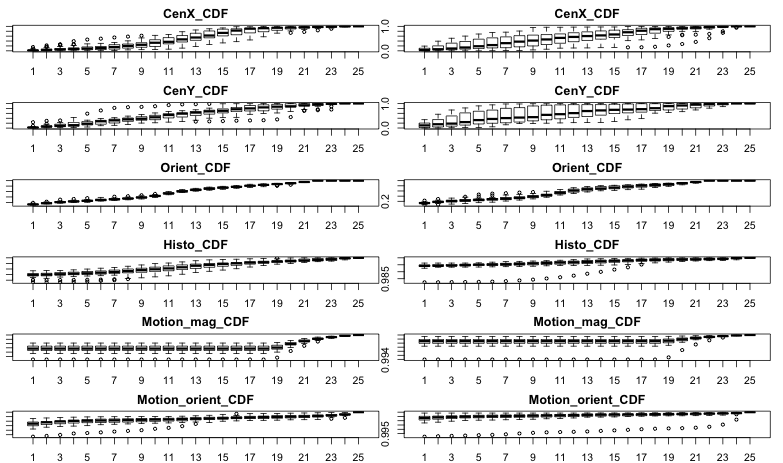
\includegraphics[width=\textwidth]{figures/writing_cdfs}
%   \caption{Box and whiskers plot of CDFs for writing. The first column represents the
%   statistics for typing and the second column represents the statistics for no
%   writing.}
% \end{figure}

\FloatBarrier

\begin{table}[h]
  \begin{centering}
  \begin{tabular}{| l | l | l |}
  \hline
   & \textbf{writing} & \textbf{no writing}\\ \hline
  \textbf{writing} & 18 & 2 \\ \hline
  \textbf{no writing} & 11 & 9 \\ \hline
  \end{tabular}
  \caption{Confusion matrix for classification accuracy for typing}
  \label{tab:writing_confusion}
\end{centering}
\end{table}

As can be seen in Table \ref{tab:writing_confusion}, we did not get as good
as results for writing, only about 65\% classification. In these results we
find that our algorithm struggled more with classifying videos that had no
writing in them as having writing in them. This may mean that the motion vectors
we are extracting are highly dependent on the type of scene we are looking at. Furthermore,
the original algorithm was developed in Matlab and then ported to C++ for this thesis. We
saw differences in the feature vectors between the two implementations; however,
classification results proved to be very similar.

\section{\label{section:scalability}Proof of Scalability}
In order to show that our system is scalable, we record the time it takes for
the cluster to perform certain repetitive tasks. For the first experiment, we
have the cluster operate using only a single EC2 instance, and then scale the
experiment by one instance and compare how long it takes to calculate 10 2.1MB
videos. For this experiment, we used Amazon's t2.micro instance which contains 1
virtual CPU running on a high frequency Intel Xeon processor with turbo up to
3.3GHz and contains 1GB of memory. Because t2 instances are designed to  have
burstable performance, Amazon does not list any specific processor on their webpage
as can be seen in Figure \ref{fig:instance_table}. Amazon designed
these instances like this so that the user is not consistently charged  for using
high performance CPUS, but rather only when they need the performance are  they
charged for those compute cycles. As a result, T2 instances can take
advantage of Intel capabilities such as native instructions for AES
encryption (AES-NI) Advanced Vector Extensions (AVX) for floating point and
Turbo Boost where the CPU core can be made to run faster. So for this reason, we
cannot give an exact chip type that was used when performing these computations
because it is possible that the virtual CPU that we were initially assigned, is
not the same CPU that we received later on in the experiment. This is the
instance that is considered to be part of the free tier program. Our instance
runs a special Amazon Machine image The results from this experiment are show in
Figure
\ref{fig:speed_up}

\begin{figure}[h]
  \label{fig:instance_table}
  \centering
  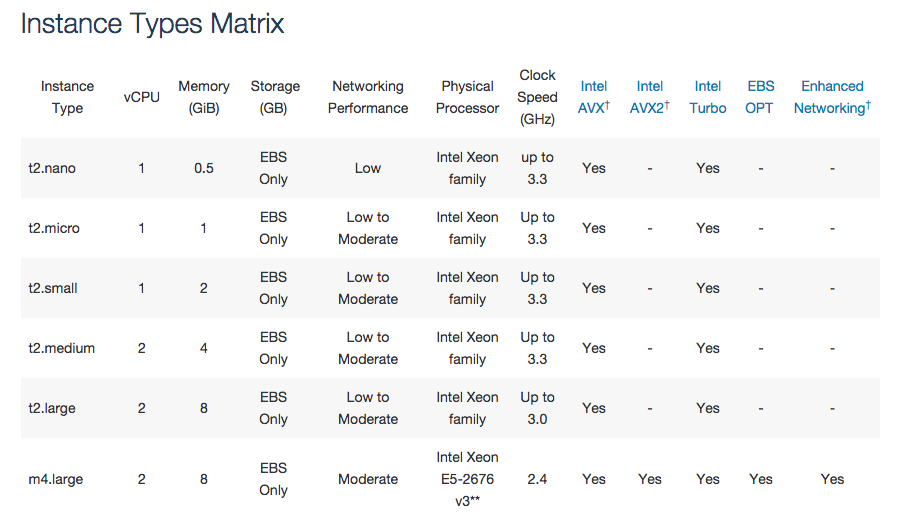
\includegraphics[width=\textwidth]{figures/instance_table}
  \caption{A subset of instances that can be used for processing on the cloud.
  Notice how t2 instances are not associated with any specific processor, only
  the processor family.}
\end{figure}

\begin{figure}[h]
  \label{fig:speed_up}
  \centering
  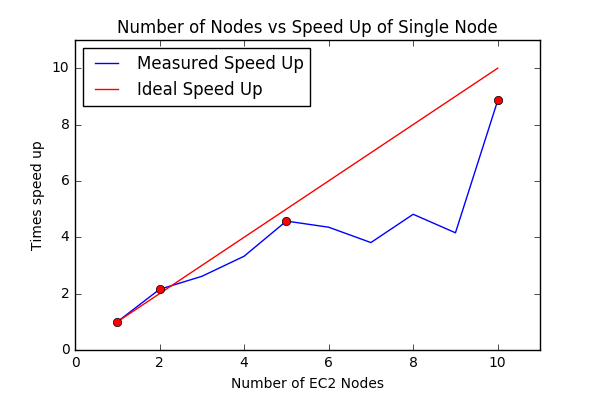
\includegraphics[width=.8\textwidth]{figures/speed_up}
  \caption{Leaving the number of videos to process the same, we increase the
  number of EC2 instances to illustrate the speed up.}
\end{figure}

From Figure \ref{fig:speed_up}, we can see that as long as the number of instances
that we have divides evenly into the number of videos that calculate, then we
get a linear increase in speed. In other words, we get 10x speed up when using
10 instances rather than just using a single instance.

The size of the videos does matter. The smaller that the videos are, the less
the overhead is when running the cluster. The reason for this is because not only
does it take longer to transfer larger videos, but it also takes more time to process
them. So from our experiments, it looks like keeping the videos under 2MB is optimal
for distributing and processing the videos.
We tested how well the t2.micro instances performed against our MacBook Pro 15 inch
with an Intel Core i7 clocked at 2.7 GHz and has 16GB of RAM. It should also be
noted that the Macbook Pro contains an AMD Radeon R9 M370X GPU with 2048 GB of
memory. This allows us to take advantage of the TAPI programming model that
we leverage as described in the Methods section.  As shown in figure \ref{fig:size_matters},
we can see that even though we have significant processing power locally, we still
must receive the message from the queue and then process the videos; therefore
there is actually little gained in terms of performance even though we are able
to leverage the onboard GPUs. Figure \ref{fig:size_matters} also demonstrates
that 10 instances run at exactly the same speed as a single instance. So from this
graph we can also infer that even though we have a higher power CPU technically
on the t2.micro instance, we are able to leverage OpenCV's transparent API and
take advantage of the local GPU on the Macbook Pro.


\begin{figure}[h]
  \centering
  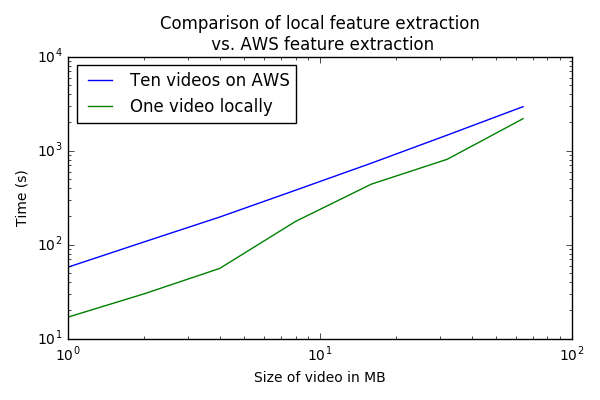
\includegraphics[width=.9\textwidth]{figures/aws_vs_local.png}
  \caption{Comparison of the time it takes for a single node to process 1 video
  vs the time it takes a cluster to process 10 videos. Videos vary in size to
  test the efficacy of choosing to send smaller vs larger videos to the cluster.
  A single t2.mirco instance was included to show that a single instance takes
  just as long as 10 instances.}
  \label{fig:size_matters}
\end{figure}

\FloatBarrier

Additionally, we can see that the performance of S3 has a linear download and upload
speed from an EC2 instance. We have collected data that calculates the mean of 10
sample download-upload pairs of a given file size. The results of this are shown
in Figures \ref{fig:s3_upload_speed} and \ref{fig:s3_download_speed}. So as expected,
we can rely on S3 to give us a linearly predictable download and upload rate.
Because though, it can take a significant time to download, process, and upload videos,
it is more beneficial for the distributed system to break videos into smaller
pieces so that no one node is occupied for a long period of time. If this
notion is followed, it is much easier to scale the feature extractions horizontally.

\begin{figure}[h]
  \centering
  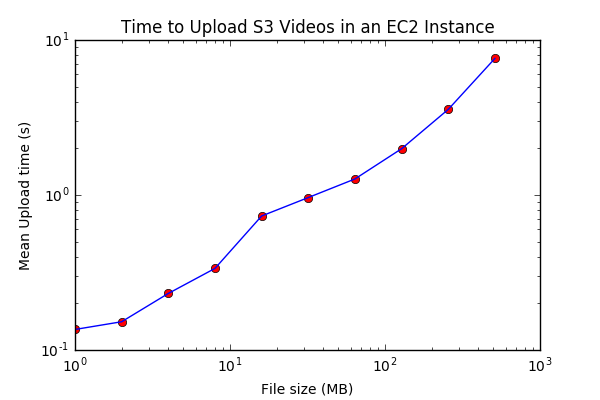
\includegraphics[width=.8\textwidth]{figures/s3_upload_speed}
  \caption{Average time to upload varying file sizes in S3 using an EC2 instance. }
  \label{fig:s3_upload_speed}
\end{figure}


The upload times can be seen in Table \ref{tab:upload_speed}
\begin{table}[h]
  \begin{tabular}{lr}
\toprule
{File Size} &         Seconds \\
\midrule
Upload 1MB (s)   &  0.135685 \\
Upload 2MB (s)   &  0.152184 \\
Upload 4MB (s)   &  0.231676 \\
Upload 8MB (s)   &  0.336037 \\
Upload 16MB (s)  &  0.732164 \\
Upload 32MB (s)  &  0.963004 \\
Upload 64MB (s)  &  1.269231 \\
Upload 128MB (s) &  1.989168 \\
Upload 256MB (s) &  3.567965 \\
Upload 512MB (s) &  7.608010 \\
\bottomrule
\end{tabular}
\caption{Average upload speeds in seconds on an EC2 instance to an S3 bucket}
\label{tab:upload_speed}
\end{table}


\begin{figure}[h]
  \centering
  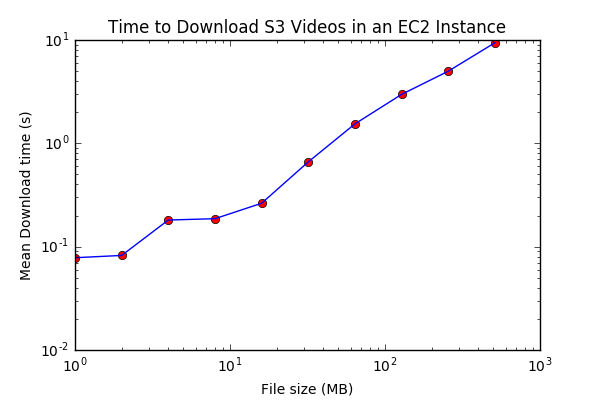
\includegraphics[width=.8\textwidth]{figures/s3_download_speed}
  \caption{Average time to download varying file sizes in S3 using an EC2 instance. }
  \label{fig:s3_download_speed}
\end{figure}

The download times can be seen in Table \ref{tab:download_speed}
\begin{table}[h]
  \begin{tabular}{lr}
  \toprule
  {File Size} &         Seconds \\
  \midrule
  Download 1MB (s)   &  0.078182 \\
  Download 2MB (s)   &  0.082242 \\
  Download 4MB (s)   &  0.181033 \\
  Download 8MB (s)   &  0.186510 \\
  Download 16MB (s)  &  0.263108 \\
  Download 32MB (s)  &  0.661547 \\
  Download 64MB (s)  &  1.542783 \\
  Download 128MB (s) &  2.976941 \\
  Download 256MB (s) &  4.990264 \\
  Download 512MB (s) &  9.406564 \\
  \bottomrule
  \end{tabular}
\caption{Average Download speeds in seconds on an EC2 instance from S3}
\label{tab:download_speed}
\end{table}


When we consolidate the numbers above, we find that we end up with an average
upload speed of 37.0486495118 MB/s and an average download speed of 40.149124154 MB/s.

\FloatBarrier

\section{Discussion}
In the previous sections we showed that we can accurately classify typing in
small segments of video and demonstrated how to we can horizontally and vertically
scale our system in the cloud. In order to achieve this, we had to find the
optimal points to break the system apart so that the computationally
expensive aspects of the system could be handled by the compute cluster, and the
quick computations could be handled by the master node, or a client node.
The quick computations in the master or client node are made possible by the
cluster of computers reducing the video files down to only a few significant
CDFs. Thus, given a set of CDFs that are only tens of kilobytes in size, we
were able to quickly train a machine learning algorithm using some ground truth
videos, and then could quickly classify features being output from the system
in microseconds.

Based on the plot in Figure \ref{fig:speed_up}, we showed that the system
we have proposed in this thesis is horizontally scalable to at least 10 nodes.
More nodes could have easily been selected, but in an attempt to keep the cost
of this thesis low, we decided to only use what is available by default in the
AWS cloud. However, based on the success of other applications, such as
Netflix that have used cloud technologies to scale their system to hundreds
or even thousands of nodes, there is no reason to believe that this system
would not scale to the same order of magnitude, though more care would probably
need to be taken to scale the nodes strategically on the AWS network services.

Finally we showed that is possible to create a greatly reduced feature space
from videos and accurately classify when students are typing at nearly 90\%.
Because the feature space is so significantly reduced after processing the
videos on the cloud, classification of videos becomes a task that takes only
milliseconds once the system has been trained. Furthermore, even training, once
the feature space has been reduced, only takes a matter of minutes for very
large datasets. As we also showed, we did not get very statistically significant
results for classifying writing. It is unclear why the motion vectors for this
activity were not as significant as they were for typing.

\subsection{Limitations}
One of the limitations of this research was retrieving sufficient ground truth
data for the videos that are analyzed. Many of the datasets that were
used in other research in this area have large datasets with ground truth
associated with them. Since the dataset we use in this paper is novel, we didn't
have the time nor the resources to generate a dataset with hundreds of samples
with ground truth.

Additionally, we were resource bound financially for this research. If we had more
money to conduct the research, we could have tested the system at a larger
scale to prove that it would work beyond just ten nodes.

Since most of the focus on this paper is primarily to investigate how to
efficiently distribute and analyze videos in the AWS cloud, there was less time
for investigation in determining the best ways to classify the human activity.
One of the short comings of this research was that it didn't address trying to
classify typing against writing. In other words, the paper doesn't investigate
classification of typing from writing, it only investigates whether we classify
a video as having typing in it, or not having typing in it.



 % But this is by no means a full implementation of the system
 % we would like to create for interactive analysis of AOLME videos. Figure
 % \ref{fig:full_system}
 %
 % \begin{figure}[h]
 %   \label{fig:full_system}
 %   \centering
 %   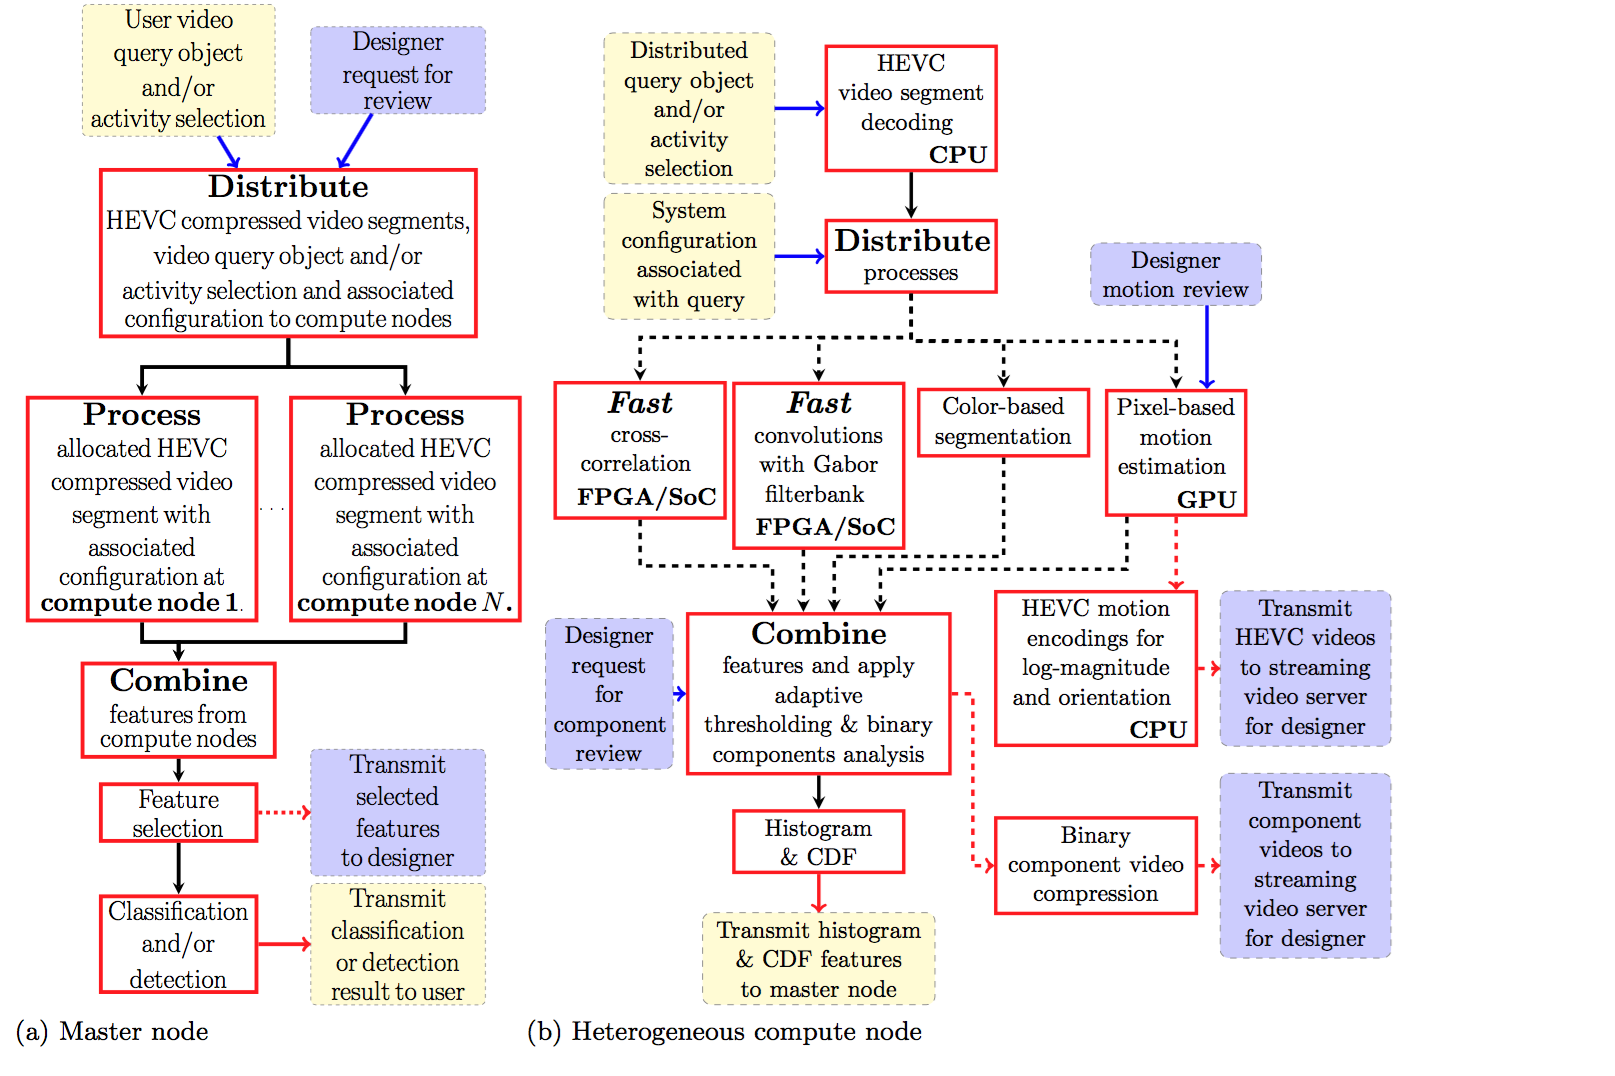
\includegraphics[width=\textwidth]{figures/full_system}
 %   \caption{Illustration of the end goal of the VIDA system. (a) shows the
 %   functions of the master node, and (b) shows the functions of the slave node.
 %   For this thesis we have implemented parts of the distribution as well as parts
 %   of the compute node.}
 % \end{figure}
 %
 % \FloatBarrier

 % For this thesis we have essentially shown that it is possible to distribute
 % small parts of the video from the master node to be consumed by the compute nodes
 % and then combined into the CDF features. We have not made the work that we have
 % done in this thesis interactive yet, but future work should be able to leverage
 % what we have done in this thesis to do so. In order to achieve the interactive
 % system that is shown in Figure \ref{fig:full_system}, we would need the master
 % node to break the HEVC videos into small 1-2MB segments to send out to the compute
 % cluster and then have the video results recombined into a single feature vector
 % when the results are collected again back at the master. This modification is
 % imperative to ensure that each one of the compute nodes can handle the workload
 % in a timely fashion. It could mean the difference between hours and minutes
 % as illustrated in Figure \ref{fig:size_matters}.

  \include{discussion}
  
\subsection{Future Work}
\PARstart This thesis investigates the basic idea how to efficiently distribute and classify
human activity in the AOLME dataset and as a result there a few areas where the
research can be greatly improved. The first suggestion to improve the in the field
of this research is to greatly increase the size of truth data for more
statistically significant data. The research done in this paper consists of 40 video
subsets, many of which contained clips from the same footage but at varying times.
Increasing this database to several hundred would improve research here.

We also didn't investigate whether we could accurately classify typing vs writing.
This would be an extension of this research that would be important so that we
could investigate if our algorithm could determine the difference between the two
activities.

In other aspect that would be worth investigating for extending this thesis,
is to attempt to add an interactive aspect to training and testing. In other words,
it would be interesting to precompute and train the machine learning algorithms
on multiple human actions and then interactively searching through the feature
space to then observe the videos that matched the classification. Work in this
area would greatly aid with the manual analysis of the AOLME videos that is
currently being done.

Finally, we found that we didn't get very good results for classifying writing.
Investigation into this would be interesting to see why the results here varied
so much from the results we obtained from typing classification. It's still unknown
why the bag of features failed to classify writing accurately as it did for typing.
As a suspicion, with no supporting evidence, it may have something to do that
general hand movement around paper is similar to that of writing, therefore the
algorithm may struggle for this reason.

\subsection{Conclusion}
We presented a novel video processing architecture and algorithm for human
activity classification in large video databases such as the AOLME dataset. Our
method is both horizontally and vertically scalable thanks to enabling
technologies in the cloud as well as convenient APIs provided by OpenCV for easy
switching between CPU and GPU implementations of Lucas-Kanade and Farneback
optical flow methods. In addition to the scalability of our system, we also
presented an accurate method for detecting typing in video segments extracted
from the AOLME dataset. Our algorithm greatly reduced the original feature space
of gigabytes down to just a few kilobytes, which makes the bandwidth limit on
the cloud very manageable. Because the output feature space is quite small
compared with the original size of the videos input into the system, training
and testing can be done very rapidly and in turn automatic classification can be
done once the system has been trained at near real-time rates. Finally, all of
the source code can be retrieved and used from our
\href{https://github.com/AcidLeroy/OpticalFlow}{Github Repo} located at
https://github.com/AcidLeroy/OpticalFlow.


  \chapter*{Appendices}

  \addcontentsline{toc}{chapter}{Appendices}
  % Next lines duplicated from .toc file and used to create mini
  % "Appendix Table of Contents," if desired:
  %\contentsline {chapter}{\numberline {A}Proving $E=MC^2$}{4}
 % \contentsline {chapter}{\numberline {B}Derivation of $A = \pi r^2$}{5}
  % End mini table of contents

  \appendix
  \chapter{\label{ap:centroids}Retrieving Centroids and Orientations from Blobs}
\begin{minted}{cpp}
void UpdateCentroidAndOrientation(const cv::Mat& thresholded_image,
                                  cv::Mat* orientations, cv::Mat* centroids) {
  cv::Mat labels, stats, current_centroids;
  cv::connectedComponentsWithStats(thzresholded_image, labels, stats,
                                   current_centroids);
  // Don't care about background centroid, hence the range.
  if (centroids->empty()) {
    current_centroids(cv::Range(1, current_centroids.rows),
                      cv::Range(0, current_centroids.cols)).copyTo(*centroids);
  } else {
    cv::vconcat(*centroids,
                current_centroids(cv::Range(1, current_centroids.rows),
                                  cv::Range(0, current_centroids.cols)),
                *centroids);
  }

  std::vector<std::vector<cv::Point>> contours;
  cv::findContours(thresholded_image, contours, cv::RETR_LIST,
                   cv::CHAIN_APPROX_NONE);
  for (size_t i = 0; i < contours.size(); ++i) {
    // Can only fit an ellipse with 5 points, skip others
    if (contours[i].size() >= 5) {
      cv::RotatedRect result = cv::fitEllipse(contours[i]);
      orientations->push_back(result.angle);
    }
  }
}
\end{minted}

  \chapter{\label{ap:dilate}Retrieving Statistics Around Motion Blob}
\begin{minted}{cpp}
/**
 * Get the histogram for the image around the motion.
 */
template <typename T>
void GetHistoAround(const T& thresholded_motion, int disk_size,
                    const T& gray_scale_image, T* bg_histogram) {
  T dialated;
  // Get disk
  T disk = cv::getStructuringElement(cv::MORPH_ELLIPSE,
                                     cv::Size(disk_size, disk_size));
  // Dilate motion to get pixels around motion
  cv::dilate(thresholded_motion, dialated, disk);
  T diff_image = dialated - thresholded_motion;
  diff_image.convertTo(diff_image, CV_8U);
  T background;
  gray_scale_image.copyTo(background, diff_image);
  // Get histogram of background intensity
  constexpr int num_bins = 25;
  constexpr float range[] = {0, 256};  // the upper boundary is exclusive
  const float* hist_range = {range};
  bool uniform = true;
  bool accumulate = false;

  T hist;
  cv::calcHist(&background, 1, 0, T(), hist, 1, &num_bins, &hist_range, uniform,
               accumulate);
  if (bg_histogram->empty()) {
    hist.copyTo(*bg_histogram);
  } else {
    (*bg_histogram) = (*bg_histogram) + hist;
  }
}
\end{minted}

  \chapter{\label{ap:google_test}Example of Google Test}

\begin{minted}{cpp}
#include "gtest/gtest.h"
#include "gmock/gmock.h"
#include "mock_reader.h"
#include "motion_estimation.h"

TEST(MotionEstimation, OnlyOneFrameInImageSequence) {
  std::shared_ptr<MockReader> mock(new MockReader{"some_file.mov"});
  MotionEstimation<MockReader, cv::Mat> me(mock);
  std::shared_ptr<cv::Mat> a_ =
      std::make_shared<cv::Mat>(cv::Mat(256, 256, CV_8U));
  cv::randu(*a_, 0, 256);
  std::shared_ptr<Image<>> frame1{new Image<>(a_)};
  EXPECT_CALL(*mock, ReadFrameMat())
      .WillOnce(Return(frame1))
      .WillOnce(Return(nullptr));

  std::shared_ptr<MockFlow> mflow{new MockFlow()};
  ASSERT_THROW(me.EstimateMotion<MockFlow>(mflow), MotionEstimationException);
}
\end{minted}

  \chapter{\label{ap:svm_classification}R Code for SVM Classification}

\begin{minted}{r}
  ClassifyFeatures <- function(VideoHists){
    NoOfSamples <- length(VideoHists$Classification)

    # Build a factor of the correct classification:
    All_cl <- unlist(VideoHists$Classification);

    # Store 1 for wrong classification and 0 for correct.
    knnResult <- rep(1, times=NoOfSamples);
    svmResult <- rep(1, times=NoOfSamples);

    # Remove classification
    no_use = c("Filename", "Classification")
    features = GetAllExcept(VideoHists, no_use)

    # Create a leave one out classification approach
    for(i in 1:NoOfSamples)
    {
      # Set up training and testing data:
      trainData = lapply(features, function(x) x[-i]) # Remove i.
      testData  = lapply(features, function(x) x[i]) # One left out.

      #Combine data
      trainData = t(CombineFeatures(trainData, names(trainData)))
      testData = t(CombineFeatures(testData, names(testData)))

      # Prepare the labels for the training set:
      #  Optimal: k=1
      knnResult[i] <- knn (trainData, testData, All_cl[-i], k=3); # 3

      #**** With tuning ****#
      tune.out=tune(svm, trainData, All_cl[-i], , kernel="linear", ranges=list(cost=c(0.0001, 0.001, 0.01, 0.1, 1, 5, 10, 100, 10000)) , scale=FALSE)
      svmResult[i] <- predict(tune.out$best.model, testData);



      #***** Without tuning *****#
  #    model <- svm(All_cl[-i] ~ ., data=trainData, scale=FALSE);
  #    svmResult[i] <- predict(model, testData);
      cat("SVM result =  ", round(svmResult), "\n");
      cat("KNN result =  ", knnResult, "\n")

    }
\end{minted}


  \bibliographystyle{acm}
  \bibliography{ivpcl_publications}

\end{document}
